\documentclass[11pt,letterpaper]{article}
\usepackage{graphicx} 
\usepackage{multirow}
\usepackage{enumitem}
\usepackage{amssymb}
\usepackage{amsmath}
\usepackage{amsthm}
\usepackage{xcolor}
\usepackage{array}
\usepackage{geometry}
\usepackage{tikz}
\usepackage{pgfplots}
\pgfplotsset{compat=1.18}
  \geometry{
    left = 15mm,
    right = 15mm,
    top = 20mm,
    bottom = 30mm,
  }
\usepackage{fancyhdr}
\renewcommand{\headrulewidth}{0pt}
\pagestyle{fancy}

\graphicspath{{C:/Users/teoso/Documents/Template Math Depart/}{D:/Hada Touya/Tugas-Kuliah/Template Math Depart/}}

\begin{document}
\pagenumbering{gobble}

\noindent
\begin{minipage}{0.15\textwidth}
  
\includegraphics[width=1.8cm]{ITS.png}
\end{minipage}%
\begin{minipage}{0.7\textwidth}
  \centering
  \textbf{EVALUASI TENGAH SEMESTER GENAP 2024 / 2025} \\
  \textbf{DEPARTEMEN MATEMATIKA - FSAD ITS} \\
  \vspace{0.3cm}
  \begin{tabular}{l l p{8cm}}
    Mata kuliah / Kode & : & Analisis Vektor / SM234405            \\
    Hari / Tanggal     & : & Selasa, 22 April 2025                 \\
    Sifat / waktu      & : & Tutup buku, 100 menit                 \\
    Dosen              & : & Dra. Nur Asiyah, M.Si.                \\
                       &   & Prof. Drs. Basuki Widodo, M.Sc., Ph.D \\
                       &   & Drs. Sentot Didik Surjanto, M.Si.     \\
                       &   & Prof. Dr. Chairul Imron, MI. Komp     \\
                       &   & Drs. Kamiran, M.Si.
  \end{tabular}
\end{minipage}%
\begin{minipage}{0.15\textwidth}
  \centering
  
\includegraphics[width=1.8cm]{M.png}
\end{minipage}

\vspace{0.5cm}

\noindent \textbf{HARAP DIPERHATIKAN !!!} \\
\textit{Segala jenis pelanggaran (mencontek, kerjasama, dsb) yang dilakukan saat ETS/EAS akan dikenakan sanksi pembatalan mata kuliah pada semester yang sedang berjalan.}

\vspace{0.5cm}

\noindent \textbf{ETS mengukur kemampuan}
\vspace*{.1cm}
\begin{center}
  \begin{tabular}{|c|p{9cm}|c|c|c|c|c|}
    \hline
    \multicolumn{2}{|c|}{\multirow{2}{*}{\textbf{CPMK}} } & \multirow{2}{*}{\textbf{\begin{tabular}{c} BOBOT \\ CPMK (\%) \end{tabular}}}                                                              & \multicolumn{4}{c|}{\textbf{CPL}}                                                             \\ \cline{4-7}
    \multicolumn{2}{|c|}{ }                               &                                                                                                                                            & \textbf{4}                        & \textbf{5}   & \textbf{8}   & \textbf{9}                  \\ \hline
    \textbf{CPMK-1}                                       & Mahasiswa mampu memahami dan menjelaskan aljabar vektor, fungsi vektor dan dapat mensketsa kurva dari fungsi vektor.                       & \textbf{5}                        & $\checkmark$ & $\checkmark$ &              &              \\ \hline
    \textbf{CPMK-2}                                       & Mahasiswa mampu menjelaskan diferensiasi fungsi vektor dan aplikasinya terkait dengan panjang busur, kelengkungan, serta aplikasi lainnya. & \textbf{15}                       & $\checkmark$ & $\checkmark$ & $\checkmark$ & $\checkmark$ \\ \hline
    \textbf{CPMK-3}                                       & Mahasiswa mampu menjelaskan Gradien, Divergensi, dan Curl dan dapat menerapkan dalam menyelesaikan integral Garis.                         & \textbf{5}                        & $\checkmark$ & $\checkmark$ &              &              \\ \hline
  \end{tabular}
\end{center}

\begin{center}
  \begin{tabular}{|c|c|c|c|c|}
    \hline
    \multirow{2}{*}{\textbf{SOAL}}                  & \multirow{2}{*}{\textbf{BOBOT SOAL (\%)}} & \multicolumn{3}{c|}{\textbf{BOBOT CPMK (\%)}}                                     \\ \cline{3-5}
                                                    &                                           & \textbf{CPMK-1}                               & \textbf{CPMK-2} & \textbf{CPMK-3} \\ \hline
    \textbf{1}                                      & \textbf{20}                               & \textbf{5}                                    &                 &                 \\ \hline
    \textbf{2}                                      & \textbf{20}                               &                                               & \textbf{5}      &                 \\ \hline
    \textbf{3}                                      & \textbf{20}                               &                                               & \textbf{5}      &                 \\ \hline
    \textbf{4}                                      & \textbf{20}                               &                                               & \textbf{5}      &                 \\ \hline
    \textbf{5}                                      & \textbf{20}                               &                                               &                 & \textbf{5}      \\ \hline
    \multicolumn{2}{|c|}{\textbf{TOTAL BOBOT CPMK}} & \textbf{5}                                & \textbf{15}                                   & \textbf{5}                        \\ \hline
  \end{tabular}
\end{center}

\vspace{0.25cm}
\begin{center}
  \underline{\textbf{SOAL}}
\end{center}

\begin{enumerate}
  \item Misalkan $P$ adalah titik yang tidak terletak pada garis $L$ yang melalui titik $Q$ dan $R$.
        \begin{enumerate}[label=\alph*.]
          \item Perlihatkan bahwa jarak $d$ dari titik $P$ ke garis $L$ adalah $d = \frac{|\vec{QR} \times \vec{QP}|}{|\vec{QR}|}$.
          \item Dapatkan jarak titik $(1, 2, 3)$ ke garis $x = 2 + t$, $y = 2 - 3t$, $z = 5t$.
        \end{enumerate}
  \item Suatu lintasan partikel diketahui dalam bentuk persamaan parametrik $x = 2\sin t + 2$, $y = 3\cos t$ dan $z = t$ dimana $t$ adalah waktu, $0 \leq t \leq 2\pi$.
        \begin{enumerate}[label=\alph*.]
          \item Dapatkan fungsi vektor lintasan partikel tersebut dan sketsa lintasannya.
          \item Dapatkan laju vektor kecepatan dan vektor percepatan pada waktu $t = \frac{\pi}{4}$.
        \end{enumerate}
  \item Diketahui kurva ruang dengan persamaan parametrik $x = t - \sin t$, $y = 1 - \cos t$ dan $z = 4\sin\left(\frac{t}{2}\right)$.
        \begin{enumerate}[label=\alph*.]
          \item Berikan ilustrasi sketsa dari kurva ruang tersebut.
          \item Carilah kelengkungan $K$ kurva tersebut ketika $t = \pi$.
        \end{enumerate}
  \item Apakah kedua persamaan garis $L_1$ dan $L_2$ berikut perpotongan?, Jelaskan! Jika berpotongan, maka dapatkan titik perpotongannya.
        \begin{align*}
          L_1: & \quad x = 6 + 4t, \quad y = 5 - 4t, \quad z = -1 + 5t \\
          L_2: & \quad x = 2 + 8t, \quad y = 4 - 3t, \quad z = 5 - t
        \end{align*}
  \item Tunjukkan bahwa
        \[ \nabla \cdot (\vec{r} f(r)) = 3f(r) + |r|\frac{df}{dr} \]
\end{enumerate}

\newpage
\begin{center}
  \textbf{SOLUSI}
\end{center}

\begin{enumerate}
  \item \begin{enumerate}[label=\alph*.]
          \item Vektor $\vec{QR}$ merupakan vektor arah dari garis $L$. Vektor $\vec{QP}$ menghubungkan titik pada garis ke titik $P$.
                \begin{center}
                  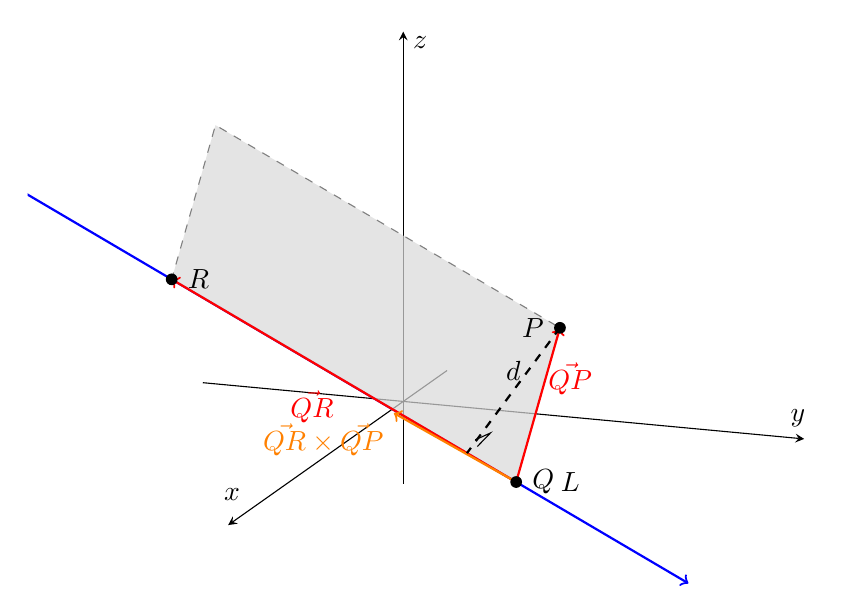
\begin{tikzpicture}
                    \begin{axis}[
                        view={110}{20}, % Sudut pandang kamera (POV) yang diubah agar jajar genjang terpisah jelas
                        width=12cm,
                        height=10cm,
                        grid=major,
                        xlabel={$x$},
                        ylabel={$y$},
                        zlabel={$z$},
                        xmin=-1, xmax=4,
                        ymin=-2, ymax=4,
                        zmin=-2, zmax=9,
                        axis lines=center,
                        ticks=none
                      ]

                      % Titik-titik
                      % Memakai titik-titik sungguhan dari soal agar gambarnya akurat secara matematis 100%
                      \coordinate (Q) at (axis cs:2,2,0);
                      \coordinate (R) at (axis cs:3,-1,5);
                      \coordinate (P) at (axis cs:1,2,3);
                      \coordinate (S) at (axis cs:2,-1,8);
                      \coordinate (P_proj) at (axis cs:2.14, 1.57, 0.71); % Titik proyeksi presisi

                      % Garis L
                      \addplot3[thick, blue, <->, forget plot] coordinates {(1.5, 3.5, -2.5) (3.5, -2.5, 7.5)} node[pos=0.2, above right, text=black] {$L$};

                      % Jajargenjang
                      \addplot3[fill=gray!30, opacity=0.7, draw=none, forget plot] coordinates {
                          (2,2,0) (3,-1,5) (2,-1,8) (1,2,3) (2,2,0)
                        };
                      \addplot3[dashed, gray, forget plot] coordinates {
                          (2,2,0) (3,-1,5) (2,-1,8) (1,2,3) (2,2,0)
                        };

                      % Vektor QR & QP
                      \draw[->, thick, red] (Q) -- (R) node[midway, below left] {$\vec{QR}$};
                      \draw[->, thick, red] (Q) -- (P) node[midway, above right] {$\vec{QP}$};

                      % Vektor cross product (Normal)
                      % Arah: (-9, -8, -3), di-scale agar muat di grafik
                      \coordinate (N) at (axis cs:-0.7, -0.4, -0.9);
                      \draw[->, thick, orange] (Q) -- (N) node[below left] {$\vec{QR} \times \vec{QP}$};

                      % Jarak d
                      \draw[dashed, thick, black] (P) -- (P_proj) node[midway, above] {$d$};

                      % Tanda Siku-siku (sudut proyeksi ke L)
                      \draw (axis cs:2.02, 1.6, 0.95) -- (axis cs:1.9, 1.7, 1.05) -- (axis cs:2.04, 1.63, 0.81);

                      % Label Titik
                      \node[circle, fill=black, inner sep=1.5pt, label=right:$Q$] at (Q) {};
                      \node[circle, fill=black, inner sep=1.5pt, label=right:$R$] at (R) {};
                      \node[circle, fill=black, inner sep=1.5pt, label=left:$P$] at (P) {};
                    \end{axis}
                  \end{tikzpicture}
                \end{center}
                Luas jajargenjang yang dibentuk oleh $\vec{QR}$ dan $\vec{QP}$ besarnya adalah $|\vec{QR} \times \vec{QP}|$. Karena Luas $=$ alas $\times$ tinggi $= |\vec{QR}| \cdot d$, maka diperoleh:
                \[ d = \frac{|\vec{QR} \times \vec{QP}|}{|\vec{QR}|} \]
          \item Diketahui titik $P(1, 2, 3)$. Garis $L$ memiliki persamaan parametrik $x = 2+t$, $y = 2-3t$, $z = 5t$.
                Titik $Q$ pada garis saat $t=0$ adalah $Q(2, 2, 0)$.
                Titik $R$ pada garis saat $t=1$ adalah $R(3, -1, 5)$.
                Vektor $\vec{QR} = \langle 1, -3, 5 \rangle$.
                Vektor $\vec{QP} = P - Q = \langle 1-2, 2-2, 3-0 \rangle = \langle -1, 0, 3 \rangle$.
                \begin{align*}
                  \vec{QR} \times \vec{QP}   & = \begin{vmatrix} \hat{i} & \hat{j} & \hat{k} \\ 1 & -3 & 5 \\ -1 & 0 & 3 \end{vmatrix} = \hat{i}(-9 - 0) - \hat{j}(3 - (-5)) + \hat{k}(0 - 3) = \langle -9, -8, -3 \rangle \\
                  |\vec{QR} \times \vec{QP}| & = \sqrt{(-9)^2 + (-8)^2 + (-3)^2} = \sqrt{81 + 64 + 9} = \sqrt{154}                                                                                                         \\
                  |\vec{QR}|                 & = \sqrt{1^2 + (-3)^2 + 5^2} = \sqrt{1 + 9 + 25} = \sqrt{35}                                                                                                                 \\
                  d                          & = \frac{\sqrt{154}}{\sqrt{35}} = \sqrt{\frac{154}{35}} = \sqrt{\frac{22}{5}}
                \end{align*}
        \end{enumerate}

  \item \begin{enumerate}[label=\alph*.]
          \item Fungsi vektor lintasan partikel adalah $\vec{r}(t) = (2\sin t + 2)\hat{i} + (3\cos t)\hat{j} + t\hat{k}$. Lintasan ini merupakan \textit{elliptical helix}.
          \item Vektor kecepatan $\vec{v}(t) = \vec{r}'(t) = 2\cos t\hat{i} - 3\sin t\hat{j} + \hat{k}$.
                Vektor percepatan $\vec{a}(t) = \vec{v}'(t) = -2\sin t\hat{i} - 3\cos t\hat{j}$.
                Pada $t = \frac{\pi}{4}$:
                \begin{align*}
                  \vec{v}\left(\frac{\pi}{4}\right)   & = 2\left(\frac{\sqrt{2}}{2}\right)\hat{i} - 3\left(\frac{\sqrt{2}}{2}\right)\hat{j} + \hat{k} = \sqrt{2}\hat{i} - \frac{3\sqrt{2}}{2}\hat{j} + \hat{k} \\
                  |\vec{v}\left(\frac{\pi}{4}\right)| & = \sqrt{(\sqrt{2})^2 + \left(-\frac{3\sqrt{2}}{2}\right)^2 + 1^2} = \sqrt{2 + \frac{18}{4} + 1} = \sqrt{3 + 4.5} = \sqrt{7.5} = \frac{\sqrt{30}}{2}    \\
                  \vec{a}\left(\frac{\pi}{4}\right)   & = -2\left(\frac{\sqrt{2}}{2}\right)\hat{i} - 3\left(\frac{\sqrt{2}}{2}\right)\hat{j} = -\sqrt{2}\hat{i} - \frac{3\sqrt{2}}{2}\hat{j}
                \end{align*}
                Jadi, laju (speed) adalah $\frac{\sqrt{30}}{2}$, dengan vektor kecepatan $\sqrt{2}\hat{i} - \frac{3\sqrt{2}}{2}\hat{j} + \hat{k}$, dan vektor percepatan $-\sqrt{2}\hat{i} - \frac{3\sqrt{2}}{2}\hat{j}$.
        \end{enumerate}

  \item \begin{enumerate}[label=\alph*.]
          \item Sketsa kurva ruang parametrik $x = t - \sin t$, $y = 1 - \cos t$, $z = 4\sin(t/2)$.
                Berikut adalah ilustrasi grafiknya dengan memetakan nilai $t$ ke koordinat 3D:
                \begin{center}
                  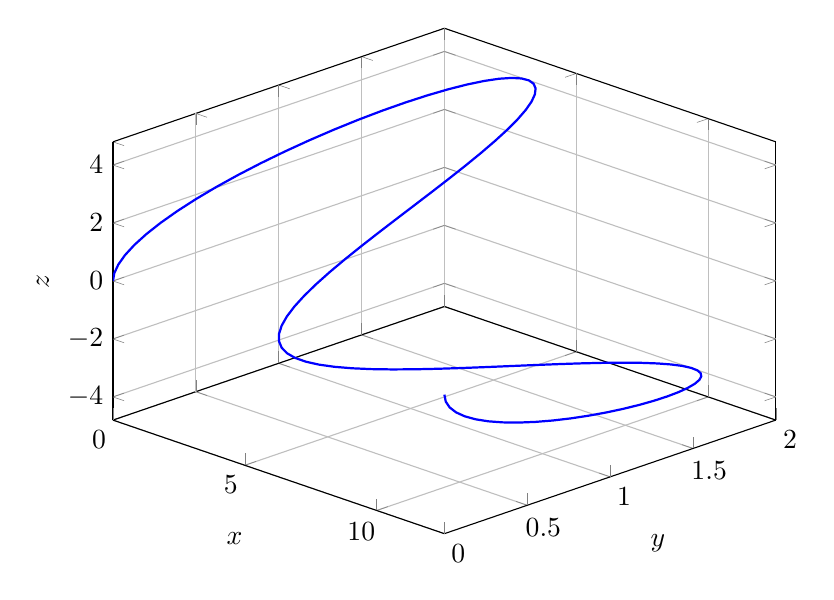
\begin{tikzpicture}
                    \begin{axis}[
                        view={45}{30},
                        width=10cm,
                        height=8cm,
                        grid=major,
                        xlabel={$x$},
                        ylabel={$y$},
                        zlabel={$z$},
                        samples=100,
                        domain=0:4*pi
                      ]
                      \addplot3 [variable=t, thick, blue, samples y=0] ({t - sin(deg(t))}, {1 - cos(deg(t))}, {4*sin(deg(t/2))});
                    \end{axis}
                  \end{tikzpicture}
                \end{center}

          \item Pada saat $t = \pi$:
                \begin{align*}
                  \vec{r}'(t)  & = \langle 1 - \cos t, \sin t, 2\cos(t/2) \rangle \\
                  \vec{r}''(t) & = \langle \sin t, \cos t, -\sin(t/2) \rangle
                \end{align*}
                Evaluasi di titik $t = \pi$:
                \begin{align*}
                  \vec{r}'(\pi)  & = \langle 1 - (-1), 0, 2(0) \rangle = \langle 2, 0, 0 \rangle \\
                  \vec{r}''(\pi) & = \langle 0, -1, -1 \rangle
                \end{align*}
                \begin{align*}
                  \vec{r}'(\pi) \times \vec{r}''(\pi)   & = \begin{vmatrix} \hat{i} & \hat{j} & \hat{k} \\ 2 & 0 & 0 \\ 0 & -1 & -1 \end{vmatrix} = \hat{i}(0-0) - \hat{j}(-2-0) + \hat{k}(-2-0) = \langle 0, 2, -2 \rangle \\
                  |\vec{r}'(\pi) \times \vec{r}''(\pi)| & = \sqrt{0^2 + 2^2 + (-2)^2} = \sqrt{8} = 2\sqrt{2}                                                                                                                \\
                  |\vec{r}'(\pi)|                       & = \sqrt{2^2 + 0 + 0} = 2
                \end{align*}
                Kelengkungan $K$:
                \[ K = \frac{|\vec{r}' \times \vec{r}''|}{|\vec{r}'|^3} = \frac{2\sqrt{2}}{2^3} = \frac{2\sqrt{2}}{8} = \frac{\sqrt{2}}{4} \]
        \end{enumerate}

  \item Untuk mengecek perpotongan secara valid, kita samakan komponen $x, y, z$ dari kedua garis menggunakan parameter yang independen ($t$ untuk $L_1$ dan $s$ untuk $L_2$):
        \begin{align*}
          L_1: & \quad x_1 = 6 + 4t, \quad y_1 = 5 - 4t, \quad z_1 = -1 + 5t \\
          L_2: & \quad x_2 = 2 + 8s, \quad y_2 = 4 - 3s, \quad z_2 = 5 - s
        \end{align*}
        Samakan koordinat $x$ dan $y$:
        \begin{align}
          6 + 4t & = 2 + 8s \implies 4t = 8s - 4 \implies t = 2s - 1 \label{eq:1} \\
          5 - 4t & = 4 - 3s \label{eq:2}
        \end{align}
        Substitusi parameter $t$ ke persamaan (\ref{eq:2}):
        \begin{align*}
          5 - 4(2s - 1) & = 4 - 3s                                \\
          5 - 8s + 4    & = 4 - 3s                                \\
          9 - 8s        & = 4 - 3s \implies 5s = 5 \implies s = 1
        \end{align*}
        Jika $s = 1$, maka diperoleh nilai $t = 2(1) - 1 = 1$.

        Selanjutnya, cek apakah dengan $s=1$ dan $t=1$, kedua garis menghasilkan nilai $z$ yang identik:
        \begin{align*}
          z_1(1) & = -1 + 5(1) = 4 \\
          z_2(1) & = 5 - (1) = 4
        \end{align*}
        Karena $z_1 = z_2 = 4$, ini membuktikan bahwa perpotongan tersebut valid secara 3 Dimensi. \textbf{Kedua garis tersebut benar-benar berpotongan}. Titik potongnya dicapai saat $t=1$ pada $L_1$, yaitu:
        \[ (x, y, z) = (6+4(1), 5-4(1), -1+5(1)) = (10, 1, 4) \]

  \item Diketahui $\vec{r} = x\hat{i} + y\hat{j} + z\hat{k}$ dan $|\vec{r}| = r = \sqrt{x^2+y^2+z^2}$.
        Maka,
        \begin{align*}
          \nabla \cdot (\vec{r} f(r)) & = \frac{\partial}{\partial x}(x f(r)) + \frac{\partial}{\partial y}(y f(r)) + \frac{\partial}{\partial z}(z f(r))                                                       \\
                                      & = \left( f(r) + x \frac{\partial f}{\partial x} \right) + \left( f(r) + y \frac{\partial f}{\partial y} \right) + \left( f(r) + z \frac{\partial f}{\partial z} \right)
        \end{align*}
        Karena $\frac{\partial r}{\partial x} = \frac{x}{r}$, maka $\frac{\partial f}{\partial x} = \frac{df}{dr} \frac{\partial r}{\partial x} = f'(r) \frac{x}{r}$. Hal yang sama berlaku untuk $y$ dan $z$.
        \begin{align*}
          \nabla \cdot (\vec{r} f(r)) & = 3f(r) + x \left( f'(r) \frac{x}{r} \right) + y \left( f'(r) \frac{y}{r} \right) + z \left( f'(r) \frac{z}{r} \right) \\
                                      & = 3f(r) + \frac{x^2+y^2+z^2}{r} f'(r)                                                                                  \\
                                      & = 3f(r) + \frac{r^2}{r} \frac{df}{dr}                                                                                  \\
                                      & = 3f(r) + r \frac{df}{dr}
        \end{align*}
        Mengingat bahwa $r = |\vec{r}|$, ini terbukti ekuivalen dengan $3f(r) + |r|\frac{df}{dr}$.
\end{enumerate}
\end{document}